\documentclass[conference]{IEEEtran}
\IEEEoverridecommandlockouts

\usepackage[utf8]{inputenc}
\usepackage[T1]{fontenc}
\usepackage{cite}
\usepackage{amsmath,amssymb,amsfonts}
\usepackage{booktabs}
\usepackage{array}
\usepackage{multirow}
\usepackage{xcolor}
\usepackage{tikz}
\usetikzlibrary{shapes.geometric,arrows.meta,positioning,fit,calc,backgrounds}
\usepackage{pgfplots}
\pgfplotsset{compat=1.18}
\usepackage[hidelinks]{hyperref}

\definecolor{pgnavy}{HTML}{1B365D}
\definecolor{pgteal}{HTML}{007A78}
\definecolor{pgamber}{HTML}{C66E00}
\definecolor{pgcrimson}{HTML}{B02A37}
\definecolor{pgslate}{HTML}{F2F5F8}
\definecolor{pgborder}{HTML}{8FA3B8}

% Helper to arrange four IEEE conference authors cleanly in a 2x2 grid
\makeatletter
\newcommand{\linebreakand}{%
  \end{@IEEEauthorhalign}
  \hfill\mbox{}\par
  \mbox{}\hfill\begin{@IEEEauthorhalign}
}
\makeatother

\begin{document}

\title{PhishGuard-Stack: Deception-Aware Multi-View URL Feature Engineering and Calibrated Dual-Modal Stacking for Fetch-Free Phishing Detection}

\author{
\IEEEauthorblockN{Kedar Kapse}
\IEEEauthorblockA{\textit{Dept. of Computer Science and Engineering}\\
\textit{School of Engineering \& Technology}\\
\textit{Pimpri Chinchwad University}, Pune, India\\
kedar.kapse24@pcu.edu.in}
\and
\IEEEauthorblockN{Ritesh Kumar}
\IEEEauthorblockA{\textit{Dept. of Computer Science and Engineering}\\
\textit{School of Engineering \& Technology}\\
\textit{Pimpri Chinchwad University}, Pune, India\\
ritesh.kumar24@pcu.edu.in}
\linebreakand
\IEEEauthorblockN{Saksham Sharma}
\IEEEauthorblockA{\textit{Dept. of Computer Science and Engineering}\\
\textit{School of Engineering \& Technology}\\
\textit{Pimpri Chinchwad University}, Pune, India\\
saksham.sharma24@pcu.edu.in}
\and
\IEEEauthorblockN{Saurabh Singh}
\IEEEauthorblockA{\textit{Dept. of Computer Science and Engineering}\\
\textit{School of Engineering \& Technology}\\
\textit{Pimpri Chinchwad University}, Pune, India\\
saurabh.singh24@pcu.edu.in}
}

\maketitle

\begin{abstract}
Credential-phishing campaigns routinely rotate through newly registered domains, free cloud preview subdomains, and Automated Certificate Management Environment (ACME) TLS certificates within hours, leaving reputation blocklists behind during initial exposure windows. Inspecting remote HTML or rendering page screenshots recovers strong visual and DOM signals, yet contacting the target server leaks defender IP telemetry, triggers server-side cloaking, and introduces network latency. Conversely, many published URL-only classifiers report inflated accuracy above 99\% due to synthetic templates or random train-test splits that leak registrable domains across partitions. We present \textbf{PhishGuard-Stack}, an end-to-end, strictly fetch-free URL screening architecture backed by a formal mathematical model and deployed across a FastAPI inference service, a React triage console, a command-line scanner, and a Chromium Manifest~V3 browser extension. Each candidate URI is mapped without network I/O into two complementary views: (i) a 48-dimensional multi-view vector capturing classical lexical counts, public-suffix-aware domain topology, homoglyph-normalized brand-domain spoofing asymmetry, bounded Levenshtein typosquatting proximity, and Dirichlet-smoothed hostname Kullback--Leibler divergence; and (ii) a sublinear TF-IDF character $n$-gram ($3 \le n \le 5$) subword representation. Four heterogeneous base learners---$L_2$ logistic regression, balanced random forest, histogram-based gradient boosted trees, and a character $n$-gram linear margin model---are fused through registrable-domain-grouped out-of-fold sigmoid meta-stacking with epistemic disagreement gating and benign-centroid instance attribution. Under strict registrable-domain-disjoint evaluation on the peer-reviewed Hannousse and Yahiouche benchmark ($11{,}429$ real URLs across $7{,}188$ unique domains; zero domain overlap), PhishGuard-Stack achieves $93.00\%$ accuracy ($95\%$ bootstrap CI: $[92.04\%, 94.09\%]$), $0.9308$ F1-score, $0.9833$ ROC-AUC, and a $0.0494$ Brier calibration score, while averaging $92.69\% \pm 0.40\%$ accuracy across five domain-disjoint folds and outperforming classical lexical baselines ($p < 10^{-7}$, McNemar's test). Zero-shot testing on $10{,}000$ unseen Ebbu2017 URLs yields $92.25\%$ accuracy ($+7.68$ percentage points over a 24-feature random forest), and zero-day screening against $300$ live 2026 OpenPhish URLs ($53.3\%$ HTTPS) detects $90.33\%$ of active attacks at $12.7$\,ms median latency.
\end{abstract}

\begin{IEEEkeywords}
phishing detection, fetch-free URL analysis, brand-spoofing divergence, calibrated stacking ensemble, domain-disjoint evaluation, browser security
\end{IEEEkeywords}

\section{Introduction}
Modern phishing infrastructure is built for disposability. Phishing-as-a-Service (PhaaS) kits automate domain registration across low-cost top-level domains (TLDs), bind wildcard TLS certificates in minutes, and stage credential harvesters behind ephemeral cloud preview hosts or dynamic DNS providers \cite{sahoo2017,prasad2024}. Curated browser blocklists remain indispensable once an abuse report propagates, yet empirical measurements repeatedly show a multi-hour gap between campaign launch and list coverage \cite{sheng2009}. During that window, the browser sees a previously unobserved Uniform Resource Identifier (URI).

Defenders confronting an unknown URI face a sharp operational trade-off. Content-driven detectors download HTML, inspect form action targets, and compare rendered page screenshots or brand logos against protected reference sets \cite{xiang2011,marchal2017,abdelnabi2020}. When page retrieval succeeds, those signals are highly diagnostic. Retrieval itself, however, carries three practical liabilities: fetching remote resources adds hundreds of milliseconds to page load, exposes client or scanner IP addresses to attacker-controlled servers, and fails silently when phishing kits serve benign decoy content to non-residential networks or headless user agents. Fetch-free URL screening operates at the opposite extreme of this design space---evaluating only the raw URI string prior to socket connection---so zero packets reach the suspect host during screening \cite{ma2009,sahingoz2019}.

Despite two decades of literature on lexical URL classification, three methodological flaws undermine how URL-only systems are typically built and evaluated:
\begin{enumerate}
\item \textit{Domain-memorization leakage and synthetic separability:} Standard random $80/20$ splits place distinct paths from the same registrable domain into both training and test sets. Tree ensembles then memorize frequent benign hostnames (or synthetic generator templates) and report near-$100\%$ test accuracy that collapses on unseen domains and deep documentation paths.
\item \textit{Protocol and naive dot-splitting bias:} Earlier lexical feature sets rely heavily on whether the scheme is \texttt{https} and count subdomain depth by splitting on dots without public-suffix awareness. Today, over half of live phishing links use valid HTTPS, while country-code second-level registries such as \texttt{.co.in}, \texttt{.ac.in}, and \texttt{.co.uk} cause naive dot counters to misclassify legitimate regional institutions.
\item \textit{Blindness to brand-ownership asymmetry:} Counting suspicious keywords or raw string lengths fails to distinguish \texttt{accounts.google.com} (authentic subdomain owned by \texttt{google.com}) from \texttt{accounts.google.com.verify-session.top} (embedded-TLD subdomain cloaking under an unrelated registrable root).
\end{enumerate}

This paper addresses all three gaps through \textbf{PhishGuard-Stack}, a mathematically formalized, fetch-free phishing detection framework paired with complete client-server deployment tooling. Specifically, our contributions are:
\begin{itemize}
\item \textbf{Multi-Layer Pre-Navigation System Architecture:} We design and implement a privacy-preserving screening architecture coupling a Manifest~V3 browser fast-path and asynchronous escalation worker, a FastAPI validation and inference engine, a React analyst dashboard, a CLI tool, and a query-redacted SQLite audit log that explicitly separates verified corporate roots from multi-tenant cloud hosting suffixes (Section~\ref{sec:arch}).
\item \textbf{Formal Deception-Aware Mathematical Model:} We formulate URI screening as a seven-tuple system $\mathcal{S}$ and derive 48 deterministic fetch-free features across four orthogonal views, introducing homoglyph-canonicalized brand-domain spoofing asymmetry $\Delta_{\text{brand}}(u)$, length-gated Levenshtein SLD typosquatting proximity $\tau_{\text{typo}}(h_{\text{sld}})$, embedded-TLD cloaking detection, and Dirichlet-smoothed hostname Kullback--Leibler divergence $D_{\text{KL}}(\tilde{P}_h \,\|\, Q)$ with linear-time complexity guarantees (Section~\ref{sec:math}).
\item \textbf{Calibrated Dual-Modal Heterogeneous Stacking:} We propose \textit{PhishGuard-Stack}, which combines three tabular learners ($L_2$ logistic regression, balanced random forest, and histogram gradient boosting) over the 48 explicit structural/deception features with a sublinear character $n$-gram ($3 \le n \le 5$) margin model via registrable-domain-disjoint out-of-fold sigmoid meta-stacking, epistemic disagreement gating, and fast benign-centroid feature attribution (Section~\ref{sec:stack}).
\item \textbf{Leakage-Free Statistical \& Cross-Corpus Validation:} We evaluate PhishGuard-Stack under strict registrable-domain-disjoint partitioning ($\mathcal{G}_{\text{train}} \cap \mathcal{G}_{\text{test}} = \emptyset$) on $11{,}429$ real URLs from Hannousse and Yahiouche \cite{hannousse2021}, benchmarking against eight standard ML classifiers and five re-implemented lexical baselines via 5-fold group cross-validation, $1{,}000$-iteration bootstrap confidence intervals, McNemar's paired significance tests, a 7-stage ablation study, $10{,}000$ unseen cross-corpus URLs from Sahingoz et al.\ \cite{sahingoz2019}, and $300$ live 2026 OpenPhish URLs (Sections~\ref{sec:setup}--\ref{sec:results}).
\end{itemize}

\section{Related Work and Research Gap}
\label{sec:related}
Research on automated phishing defense spans four primary paradigms. First, reputation blocklists such as Google Safe Browsing and PhishTank achieve near-zero false positives on previously verified URLs \cite{whittaker2010}, yet Sheng et al.\ demonstrated that reactive feeds miss a substantial fraction of short-lived campaigns at hour zero \cite{sheng2009}. Second, content and DOM inspection frameworks---most notably CANTINA+ \cite{xiang2011}, Off-the-Hook \cite{marchal2017}, Hannousse and Yahiouche's hybrid web-page features \cite{hannousse2021}, and PhiUSIIL \cite{prasad2024}---combine URI cues with HTML form tags, external hyperlink ratios, and WHOIS metadata. Third, visual similarity engines such as VisualPhishNet \cite{abdelnabi2020} match page screenshots or brand logos against protected target templates. Both content and visual systems achieve high accuracy when pages render cleanly, but require outbound HTTP requests and headless rendering that violate zero-contact privacy constraints.

Fourth, fetch-free lexical URL detectors classify strings prior to network resolution. Garera et al.\ \cite{garera2007} introduced hand-crafted host, keyword, and obfuscation indicators with logistic regression. Ma et al.\ \cite{ma2009} scaled sparse lexical bag-of-tokens models across tens of thousands of URLs, while Verma and Dyer \cite{verma2015} examined character-distribution statistics such as Kolmogorov--Smirnov divergence. Feroz and Mengel \cite{feroz2015} combined 15 structural count and length primitives with tree classifiers, and Sahingoz et al.\ \cite{sahingoz2019} benchmarked NLP token counts and random forests on the Ebbu2017 dataset. Deep character architectures including Bahnsen et al.'s recurrent network \cite{bahnsen2017} and URLNet \cite{le2018} learn subword embeddings directly from raw strings, trading interpretability and CPU efficiency for subword flexibility.

\begin{table*}[t]
\caption{Architectural and Methodological Comparison of Representative Phishing Detection Systems}
\label{tab:litgap}
\centering
\footnotesize
\renewcommand{\arraystretch}{1.15}
\resizebox{\textwidth}{!}{%
\begin{tabular}{p{2.9cm}ccccp{4.8cm}}
\toprule
\textbf{System / Study} & \textbf{Zero Network Fetch} & \textbf{Domain-Disjoint Split} & \textbf{Brand-Owner Asymmetry} & \textbf{Calibrated + Explainable} & \textbf{Key Operational Limitation} \\
\midrule
Garera et al.\ \cite{garera2007} & \checkmark & $\times$ & Partial (binary) & $\times$ & Small 8-cue linear model misses modern HTTPS \& compound spoofs \\
Ma et al.\ \cite{ma2009} & Partial (DNS/WHOIS) & $\times$ & $\times$ & $\times$ & Relies on WHOIS/ASN lookups; high-dimensional uncalibrated bag-of-words \\
Feroz \& Mengel \cite{feroz2015} & \checkmark & $\times$ & $\times$ & $\times$ & Count-only features misclassify deep benign documentation URLs \\
Sahingoz et al.\ \cite{sahingoz2019} & \checkmark & $\times$ & $\times$ & $\times$ & Naive dot splitting; 2017 corpus exhibits severe HTTP/HTTPS class skew \\
URLNet (Le et al.) \cite{le2018} & \checkmark & $\times$ & $\times$ & $\times$ & CNN black-box without probability calibration or brand-ownership logic \\
CANTINA+ / PhiUSIIL \cite{xiang2011,prasad2024} & $\times$ (Fetches DOM) & $\times$ & Partial (DOM title) & $\times$ & Contacts suspect server; vulnerable to cloaking and high page-load latency \\
\midrule
\textbf{PhishGuard-Stack (Ours)} & \textbf{\checkmark} & \textbf{\checkmark} & \textbf{\checkmark ($\Delta_{\text{brand}}, \tau_{\text{typo}}$)} & \textbf{\checkmark (OOF + $\psi_j$)} & Cannot inspect malicious forms hosted inside clean SaaS form builders \\
\bottomrule
\end{tabular}%
}
\end{table*}

Table~\ref{tab:litgap} summarizes where existing approaches fall short. Classical lexical models lack public-suffix-aware brand-ownership verification and probability calibration, whereas deep character models sacrifice instance-level auditability. Crucially, prior lexical studies rarely enforce registrable-domain-disjoint evaluation, masking overfitting to recurring domains. PhishGuard-Stack bridges explicit deception modeling and subword morphology within a strictly domain-disjoint, calibrated, fetch-free ensemble.

\section{Proposed System Architecture}
\label{sec:arch}

\begin{figure*}[t]
\centering
\resizebox{\textwidth}{!}{%
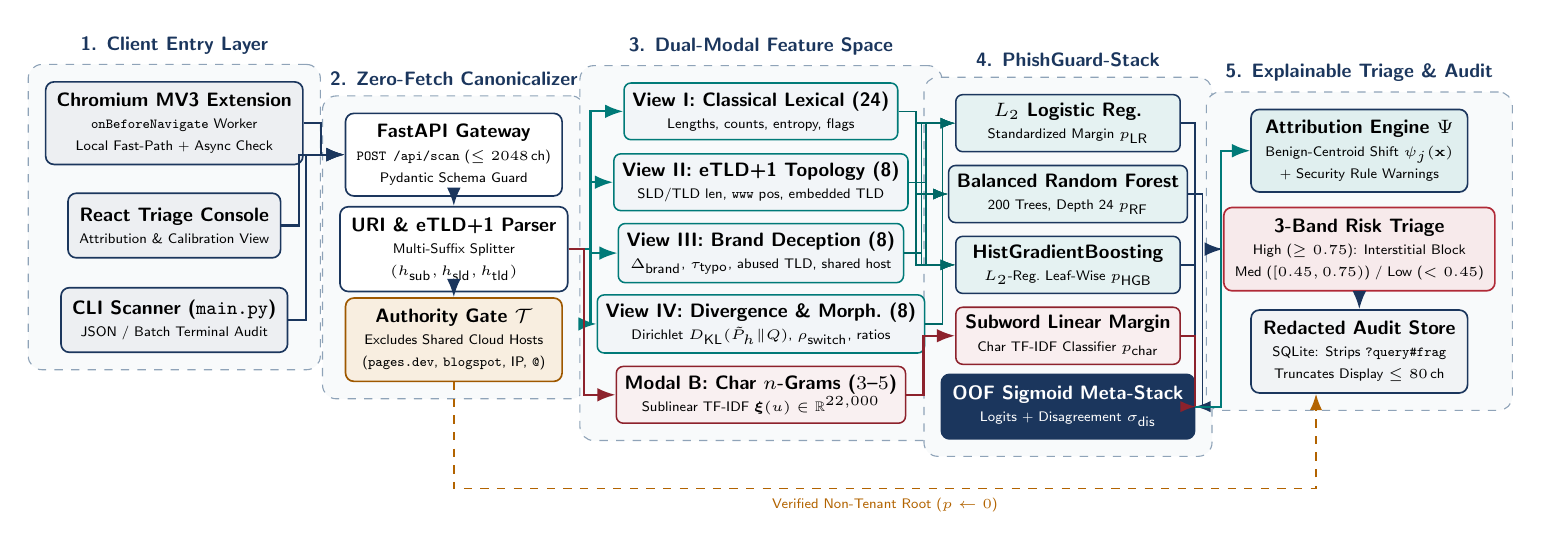
\begin{tikzpicture}[
    font=\scriptsize\sffamily,
    >=Latex,
    box/.style={draw=pgnavy, rounded corners=3pt, fill=white, minimum height=0.82cm, align=center, inner sep=4pt, line width=0.6pt},
    viewbox/.style={draw=pgteal, rounded corners=2.5pt, fill=pgslate, minimum height=0.72cm, minimum width=3.15cm, align=center, inner sep=3pt, line width=0.55pt},
    modelbox/.style={draw=pgnavy, rounded corners=2.5pt, fill=pgteal!10, minimum height=0.70cm, minimum width=2.85cm, align=center, inner sep=3pt, line width=0.55pt},
    stagebg/.style={draw=pgborder, dashed, rounded corners=5pt, fill=pgslate!55, inner sep=6pt}
]

% Column 1: Clients
\node[box, fill=pgnavy!8, minimum width=2.7cm] (ext) at (0, 1.55) {\textbf{Chromium MV3 Extension}\\{\tiny \texttt{onBeforeNavigate} Worker}\\{\tiny Local Fast-Path + Async Check}};
\node[box, fill=pgnavy!8, minimum width=2.7cm] (ui)  at (0, 0.25) {\textbf{React Triage Console}\\{\tiny Attribution \& Calibration View}};
\node[box, fill=pgnavy!8, minimum width=2.7cm] (cli) at (0, -0.95) {\textbf{CLI Scanner (\texttt{main.py})}\\{\tiny JSON / Batch Terminal Audit}};

\begin{scope}[on background layer]
  \node[stagebg, fit=(ext)(ui)(cli), label={[font=\scriptsize\bfseries\sffamily, text=pgnavy]above:1. Client Entry Layer}] (g1) {};
\end{scope}

% Column 2: API & Canonicalizer
\node[box, minimum width=2.75cm] (api) at (3.55, 1.15) {\textbf{FastAPI Gateway}\\{\tiny \texttt{POST /api/scan} ($\le 2048$\,ch)}\\{\tiny Pydantic Schema Guard}};
\node[box, minimum width=2.75cm] (psl) at (3.55, -0.05) {\textbf{URI \& eTLD+1 Parser}\\{\tiny Multi-Suffix Splitter}\\{\tiny $(h_{\text{sub}}, h_{\text{sld}}, h_{\text{tld}})$}};
\node[box, fill=pgamber!12, draw=pgamber!80!black, minimum width=2.75cm] (trust) at (3.55, -1.20) {\textbf{Authority Gate $\mathcal{T}$}\\{\tiny Excludes Shared Cloud Hosts}\\{\tiny (\texttt{pages.dev}, \texttt{blogspot}, IP, \texttt{@})}};

\begin{scope}[on background layer]
  \node[stagebg, fit=(api)(psl)(trust), label={[font=\scriptsize\bfseries\sffamily, text=pgnavy]above:2. Zero-Fetch Canonicalizer}] (g2) {};
\end{scope}

% Column 3: Dual-Modal Feature Engine
\node[viewbox] (v1) at (7.45, 1.70) {\textbf{View I: Classical Lexical (24)}\\{\tiny Lengths, counts, entropy, flags}};
\node[viewbox] (v2) at (7.45, 0.80) {\textbf{View II: eTLD+1 Topology (8)}\\{\tiny SLD/TLD len, \texttt{www} pos, embedded TLD}};
\node[viewbox] (v3) at (7.45, -0.10) {\textbf{View III: Brand Deception (8)}\\{\tiny $\Delta_{\text{brand}}$, $\tau_{\text{typo}}$, abused TLD, shared host}};
\node[viewbox] (v4) at (7.45, -1.00) {\textbf{View IV: Divergence \& Morph.\ (8)}\\{\tiny Dirichlet $D_{\text{KL}}(\tilde{P}_h\|Q)$, $\rho_{\text{switch}}$, ratios}};
\node[viewbox, draw=pgcrimson!80!black, fill=pgcrimson!7] (vc) at (7.45, -1.90) {\textbf{Modal B: Char $n$-Grams ($3$--$5$)}\\{\tiny Sublinear TF-IDF $\boldsymbol{\xi}(u) \in \mathbb{R}^{22{,}000}$}};

\begin{scope}[on background layer]
  \node[stagebg, fit=(v1)(v2)(v3)(v4)(vc), label={[font=\scriptsize\bfseries\sffamily, text=pgnavy]above:3. Dual-Modal Feature Space}] (g3) {};
\end{scope}

% Column 4: PhishGuard-Stack Ensemble
\node[modelbox] (mlr)  at (11.35, 1.55) {\textbf{$L_2$ Logistic Reg.}\\{\tiny Standardized Margin $p_{\text{LR}}$}};
\node[modelbox] (mrf)  at (11.35, 0.65) {\textbf{Balanced Random Forest}\\{\tiny 200 Trees, Depth 24 $p_{\text{RF}}$}};
\node[modelbox] (mhgb) at (11.35, -0.25) {\textbf{HistGradientBoosting}\\{\tiny $L_2$-Reg.\ Leaf-Wise $p_{\text{HGB}}$}};
\node[modelbox, draw=pgcrimson!80!black, fill=pgcrimson!8] (mch) at (11.35, -1.15) {\textbf{Subword Linear Margin}\\{\tiny Char TF-IDF Classifier $p_{\text{char}}$}};
\node[box, fill=pgnavy, text=white, minimum width=2.85cm] (meta) at (11.35, -2.05) {\textbf{OOF Sigmoid Meta-Stack}\\{\tiny Logits + Disagreement $\sigma_{\text{dis}}$}};

\begin{scope}[on background layer]
  \node[stagebg, fit=(mlr)(mrf)(mhgb)(mch)(meta), label={[font=\scriptsize\bfseries\sffamily, text=pgnavy]above:4. PhishGuard-Stack}] (g4) {};
\end{scope}

% Column 5: Attribution, Triage & Storage
\node[box, fill=pgteal!12, minimum width=2.75cm] (attr) at (15.05, 1.20) {\textbf{Attribution Engine $\Psi$}\\{\tiny Benign-Centroid Shift $\psi_j(\mathbf{x})$}\\{\tiny + Security Rule Warnings}};
\node[box, fill=pgcrimson!10, draw=pgcrimson, minimum width=2.75cm] (band) at (15.05, -0.05) {\textbf{3-Band Risk Triage}\\{\tiny High ($\ge 0.75$): Interstitial Block}\\{\tiny Med ($[0.45,0.75)$) / Low ($<0.45$)}};
\node[box, fill=pgnavy!6, minimum width=2.75cm] (db)   at (15.05, -1.35) {\textbf{Redacted Audit Store}\\{\tiny SQLite: Strips \texttt{?query\#frag}}\\{\tiny Truncates Display $\le 80$\,ch}};

\begin{scope}[on background layer]
  \node[stagebg, fit=(attr)(band)(db), label={[font=\scriptsize\bfseries\sffamily, text=pgnavy]above:5. Explainable Triage \& Audit}] (g5) {};
\end{scope}

% Arrows
\draw[->, thick, pgnavy] (ext.east) -- ++(0.22,0) |- (api.west);
\draw[->, thick, pgnavy] (ui.east)  -- ++(0.22,0) |- (api.west);
\draw[->, thick, pgnavy] (cli.east) -- ++(0.22,0) |- (api.west);

\draw[->, thick, pgnavy] (api.south) -- (psl.north);
\draw[->, thick, pgnavy] (psl.south) -- (trust.north);

\draw[->, thick, pgteal] (psl.east) -- ++(0.28,0) |- (v1.west);
\draw[->, thick, pgteal] (psl.east) -- ++(0.28,0) |- (v2.west);
\draw[->, thick, pgteal] (psl.east) -- ++(0.28,0) |- (v3.west);
\draw[->, thick, pgteal] (psl.east) -- ++(0.28,0) |- (v4.west);
\draw[->, thick, pgcrimson!80!black] (psl.east) -- ++(0.20,0) |- (vc.west);

\foreach \v in {v1,v2,v3,v4} {
  \draw[->, pgteal!85!black, line width=0.5pt] (\v.east) -- ++(0.22,0) |- (mlr.west);
  \draw[->, pgteal!85!black, line width=0.5pt] (\v.east) -- ++(0.22,0) |- (mrf.west);
  \draw[->, pgteal!85!black, line width=0.5pt] (\v.east) -- ++(0.22,0) |- (mhgb.west);
}
\draw[->, thick, pgcrimson!80!black] (vc.east) -- ++(0.22,0) |- (mch.west);

\draw[->, pgnavy, line width=0.55pt] (mlr.east)  -- ++(0.18,0) |- (meta.east);
\draw[->, pgnavy, line width=0.55pt] (mrf.east)  -- ++(0.18,0) |- (meta.east);
\draw[->, pgnavy, line width=0.55pt] (mhgb.east) -- ++(0.18,0) |- (meta.east);
\draw[->, pgcrimson!80!black, line width=0.55pt] (mch.east) -- ++(0.18,0) |- (meta.east);

\draw[->, thick, pgnavy] (meta.east) -- ++(0.32,0) |- (band.west);
\draw[->, thick, pgteal] (meta.east) -- ++(0.32,0) |- (attr.west);
\draw[->, thick, pgnavy] (band.south) -- (db.north);
\draw[->, dashed, pgamber!90!black, line width=0.65pt] (trust.south) -- ++(0,-1.35) -| node[pos=0.25, below, font=\tiny\sffamily]{Verified Non-Tenant Root ($p \leftarrow 0$)} ([xshift=-0.55cm]db.south);

\end{tikzpicture}%
}
\caption{Proposed \textbf{PhishGuard-Stack} five-stage system architecture. Candidate URLs never trigger outbound DNS, TCP, or HTTP requests to the suspect server; structural/deception views ($\Phi_{\text{I}}$--$\Phi_{\text{IV}} \in \mathbb{R}^{48}$) and subword character $n$-grams ($\boldsymbol{\xi}(u)$) are fused via domain-grouped out-of-fold calibrated stacking.}
\label{fig:arch}
\end{figure*}

Figure~\ref{fig:arch} illustrates the five-stage architecture of PhishGuard-Stack. Every component enforces a strict \emph{zero-remote-touch} invariant: neither the browser worker nor the FastAPI backend resolves DNS records, opens TLS handshakes, or downloads HTML from the candidate address.

\subsection{Threat Model and Trust Boundary}
We consider an adversary who controls arbitrary domain registrations, unlimited subdomain prefixes, URL paths, query parameters, and valid DV/ACME TLS certificates, and who may host phishing pages on shared cloud preview or free web-hosting platforms (e.g., \texttt{pages.dev}, \texttt{web.app}, \texttt{firebaseapp.com}, \texttt{000webhostapp.com}, \texttt{blogspot.com}, or dynamic DNS suffixes). Attackers systematically imitate trusted brands via subdomain nesting (\texttt{paypal.com.verify-acct.top}), leetspeak homoglyphs (\texttt{paypa1-secure.tk}), Punycode IDN labels (\texttt{xn--...}), or RFC~3986 \texttt{userinfo@} syntax \cite{rfc3986}.

To prevent false alarms on complex search or documentation URLs belonging to major global platforms without opening a loophole for cloud-hosted phishing, our Authority Gate ($\mathcal{T}$) enforces a two-step exclusion rule. First, any host matching a curated registry of 43 multi-tenant cloud, free-hosting, tunneling, or dynamic-DNS suffixes ($\mathcal{H}_{\text{shared}}$) is immediately disqualified from allow-listing and flagged via \texttt{free\_hosting\_host=1}. Second, only exact matches or authentic subdomains of 54 high-reputation non-tenant roots ($\mathcal{T}_{\text{root}}$, such as \texttt{python.org}, \texttt{google.com}, or \texttt{ieee.org}) lacking raw IP literals and \texttt{@} symbols bypass classification. Compromised pages hosted directly inside a clean third-party domain whose URL string exhibits no lexical anomalies remain outside the theoretical observability of URL-only screening; we quantify such cases explicitly in Section~\ref{sec:errors}.

\subsection{Two-Stage Browser Pre-Navigation Guard and Privacy Store}
In Chromium Manifest~V3, \texttt{webNavigation.onBeforeNavigate} fires before a top-level frame commits, but does not pause the browser's network stack while awaiting an asynchronous HTTP call. Claiming synchronous network blocking for a remote ML call would therefore be inaccurate. Instead, our service worker implements a two-stage pipeline: Stage~1 executes an inline JavaScript lexical rule evaluator in under $0.2$\,ms that immediately redirects blatantly deceptive navigations (raw IPv4/IPv6 login paths, \texttt{userinfo@} cloaking, or embedded-TLD brand spoofing on abused TLDs) to a local interstitial warning page (\texttt{blocked.html}) before connection setup. Stage~2 asynchronously posts remaining URLs to the local FastAPI endpoint (\texttt{POST /api/scan}); if PhishGuard-Stack returns high risk ($p \ge 0.75$), the active tab is redirected upon response arrival ($\sim 14$\,ms local round-trip). Users retain a per-domain session override.

Because query strings and URI fragments routinely carry OAuth codes, session identifiers, or personal tokens, the persistence layer strips everything following \texttt{?} or \texttt{\#} and truncates the display string to 80 characters prior to parameterized SQLite insertion.

\section{Formal Mathematical Model}
\label{sec:math}

\subsection{Set-Theoretic System Formulation}
We formalize PhishGuard-Stack as a deterministic seven-tuple screening machine:
\begin{equation}
\mathcal{S} = \langle \mathcal{U},\, \mathcal{T},\, \Phi,\, \mathcal{G}_{\text{char}},\, \mathcal{M},\, \mathcal{C},\, \Psi \rangle,
\label{eq:tuple}
\end{equation}
where $\mathcal{U} \subseteq \Sigma^{\le 2048}$ denotes the space of bounded URI strings over printable ASCII/UTF-8 alphabet $\Sigma$; $\mathcal{T}: \mathcal{U} \to \{0,1\}$ is the shared-host-aware authority predicate; $\Phi: \mathcal{U} \to \mathbb{R}^{48}$ maps each URI into four structured feature views $\Phi(u) = [\Phi_{\text{I}}(u) \,\|\, \Phi_{\text{II}}(u) \,\|\, \Phi_{\text{III}}(u) \,\|\, \Phi_{\text{IV}}(u)]^\top$; $\mathcal{G}_{\text{char}}: \mathcal{U} \to \mathbb{R}^{V}$ extracts sublinear TF-IDF character $n$-gram weights ($V \le 22{,}000$); $\mathcal{M} = \{f_{\text{LR}}, f_{\text{RF}}, f_{\text{HGB}}, f_{\text{char}}\}$ is the heterogeneous base-learner bank; $\mathcal{C}: [0,1]^4 \to [0,1]$ is the out-of-fold calibrated sigmoid meta-combiner producing calibrated posterior $\hat{p}(y=1 \mid u)$; and $\Psi: \mathbb{R}^{48} \to \mathbb{R}^{48}$ computes signed instance-level feature attributions.

\subsection{Public-Suffix-Aware URI Decomposition (View II)}
Given a raw string $u \in \mathcal{U}$, RFC~3986 parsing extracts scheme $s$, authority host $h$ (lowercased, port-stripped), path $p$, query $q$, and fragment $r$ \cite{rfc3986}. Naive dot-splitting treats two-level country registries such as \texttt{www.sbi.co.in} as having two subdomains above registrable root \texttt{co.in}. Let $\mathcal{E}_{2}$ denote our curated set of 52 multi-label effective public suffixes (e.g., \texttt{co.in}, \texttt{ac.in}, \texttt{gov.in}, \texttt{co.uk}, \texttt{com.au}, \texttt{co.jp}). Splitting non-IP host $h$ into dot-separated labels $(l_1, l_2, \dots, l_k)$, the canonical decomposition $(h_{\text{sub}}, h_{\text{sld}}, h_{\text{tld}})$ is defined as:
\begin{equation}
\resizebox{0.89\columnwidth}{!}{$\displaystyle
(h_{\text{sub}}, h_{\text{sld}}, h_{\text{tld}}) =
\begin{cases}
(l_{1..k-3},\, l_{k-2},\, l_{k-1}.l_k), & k \ge 3,\; l_{k-1}.l_k \in \mathcal{E}_{2}, \\
(l_{1..k-2},\, l_{k-1},\, l_k), & k \ge 2,\; l_{k-1}.l_k \notin \mathcal{E}_{2}.
\end{cases}$}
\label{eq:etld}
\end{equation}
The canonical registrable domain is $g(u) = h_{\text{sld}}.h_{\text{tld}}$ (or tenant-qualified $l_{k_{\text{sub}}}.h_{\text{sld}}.h_{\text{tld}}$ when $h$ suffixes $\mathcal{H}_{\text{shared}}$). View~II records $|h_{\text{sld}}|$, $|h_{\text{tld}}|$, canonical \texttt{www} presence $\mathbb{I}[l_1 = \text{\texttt{www}}]$, misplaced \texttt{www} $\mathbb{I}[\text{\texttt{www}} \in h_{\text{sld}} \lor \text{\texttt{www}} \in l_{2..}]$, path segment depth, longest alphanumeric token length, host-to-URL length ratio $|h|/|u|$, and embedded-TLD cloaking $\mathbb{I}[\exists t \in \text{tok}(h_{\text{sub}}) \cup \text{split}_{'-'}(h_{\text{sld}}) : t \in \{\text{\texttt{com, net, org, edu, gov, io, co, uk}}\}]$.

\subsection{Homoglyph Brand-Spoofing Asymmetry \& Typosquatting (View III)}
Attackers frequently substitute visually confusable glyphs (\texttt{0}$\to$\texttt{o}, \texttt{1}$\to$\texttt{l}/\texttt{i}, \texttt{3}$\to$\texttt{e}, \texttt{4}$\to$\texttt{a}, \texttt{5}$\to$\texttt{s}, \texttt{rn}$\to$\texttt{m}, \texttt{vv}$\to$\texttt{w}) to impersonate high-value brands while registering an unrelated root $h_{\text{sld}}$. Let $\Gamma(t)$ denote the set of canonicalized homoglyph projections of token $t$, and let $\mathcal{B}$ be a curated lexicon of 48 target brands where each brand $b \in \mathcal{B}$ is paired with its authorized sibling SLD set $\Omega(b)$ (for example, $\Omega(\text{\texttt{google}}) = \{\text{\texttt{google}},\allowbreak \text{\texttt{googleapis}},\allowbreak \text{\texttt{gstatic}},\allowbreak \text{\texttt{youtube}},\allowbreak \text{\texttt{gmail}}\}$). For any token $t$ and brand $b$, the length-gated visual similarity $\kappa(t, b)$ is:
\begin{equation}
\resizebox{0.89\columnwidth}{!}{$\displaystyle
\kappa(t, b) = \max_{v \in \Gamma(t)}
\begin{cases}
1.00, & t = b, \\
0.96, & t \neq b \land v = b, \\
1 - \dfrac{d_{\text{lev}}(v, b)}{\max(|v|, |b|)}, & d_{\text{lev}}(v,b) \le \delta(|v|,|b|), \\
0, & \text{otherwise},
\end{cases}$}
\label{eq:brandsim}
\end{equation}
where $d_{\text{lev}}$ is Levenshtein edit distance and $\delta(\ell_1,\ell_2) = 2$ if $\min(\ell_1,\ell_2) \ge 8$, $1$ if $5 \le \min(\ell_1,\ell_2) < 8$, and $0$ otherwise, excluding common benign English collisions (e.g., \emph{apply}, \emph{stream}). Defining effective owner $\tilde{o}(u) = \varnothing$ if $h \in \mathcal{H}_{\text{shared}}$ else $h_{\text{sld}}$, we define \textbf{Brand-Domain Spoofing Divergence} $\Delta_{\text{brand}}(u)$ across host tokens $\mathcal{W}_{\text{host}}(u)$ and path tokens $\mathcal{W}_{\text{path}}(u)$ (with exact/homoglyph matching on paths, weighted by $\gamma = 0.90$):
\begin{equation}
\begin{aligned}
\Delta_{\text{brand}}(u) = \!\max_{\substack{b \in \mathcal{B} \\ \tilde{o}(u) \notin \Omega(b)}}\! \max\Big(
  &\max_{t \in \mathcal{W}_{\text{host}}} \kappa(t,b), \\[-2pt]
  &\gamma \max_{t \in \mathcal{W}_{\text{path}}} \mathbb{I}[\kappa(t,b) \ge 0.96]\kappa(t,b) \Big).
\end{aligned}
\label{eq:spoof}
\end{equation}
Similarly, \textbf{SLD Typosquatting Proximity} $\tau_{\text{typo}}(h_{\text{sld}})$ measures direct look-alike registration on the second-level label itself:
\begin{equation}
\tau_{\text{typo}}(h_{\text{sld}}) = \max_{\substack{b \in \mathcal{B},\; \tilde{o}(u) \notin \Omega(b) \\ c \in \{h_{\text{sld}},\, h_{\text{sld}}^{-}\} \,:\, c \neq b \lor \text{`-'}\in h_{\text{sld}}}} \kappa(c, b),
\label{eq:typo}
\end{equation}
where $h_{\text{sld}}^{-}$ strips hyphens to catch compound spoofs such as \texttt{pay-pal.com}. Under (\ref{eq:spoof})--(\ref{eq:typo}), legitimate \texttt{accounts.google.com} yields $\Delta_{\text{brand}}=0$ because $h_{\text{sld}}=\text{\texttt{google}} \in \Omega(\text{\texttt{google}})$, whereas \texttt{accounts.google.com.verify-session.top} yields $\Delta_{\text{brand}}=1.00$ because $h_{\text{sld}}=\text{\texttt{verify-session}} \notin \Omega(\text{\texttt{google}})$.

\subsection{Dirichlet-Smoothed KL-Divergence \& Morphology (View IV)}
Algorithmically generated subdomains and randomized phishing slugs deviate from the character distribution $Q$ of natural domain names, yet raw maximum-likelihood character probabilities suffer severe finite-sample inflation on short benign domains (e.g., three-letter acronyms). Stripping leading \texttt{www.} to obtain $h_{\text{core}}$ with $n = |h_{\text{core}}|$ alphanumeric characters and count $c_a$ for symbol $a \in \mathcal{A}_{36}$, we place a Dirichlet prior of concentration $\alpha = 5.0$ centered on empirical benign prior $Q$:
\begin{equation}
\begin{aligned}
\tilde{P}_{h}(a) &= \frac{c_a + \alpha Q(a)}{n + \alpha}, \\
D_{\text{KL}}\!\left(\tilde{P}_h \,\middle\|\, Q\right) &= \sum_{a \in \mathcal{A}_{36}} \tilde{P}_h(a) \log_2 \frac{\tilde{P}_h(a)}{Q(a)}.
\end{aligned}
\label{eq:kl}
\end{equation}
As $n \to 0$, $\tilde{P}_h \to Q$ and $D_{\text{KL}} \to 0$, preventing false penalties on concise domains while preserving strong divergence on long pseudo-random strings. View~IV complements $D_{\text{KL}}$ with path Shannon entropy $H(p) = -\sum_c \hat{p}(c)\log_2 \hat{p}(c)$ \cite{shannon1948}, character-class transition rate
\begin{equation}
\rho_{\text{switch}}(h) = \frac{1}{\max(|h|-1, 1)} \sum_{i=1}^{|h|-1} \mathbb{I}\!\left[\pi(h_i) \neq \pi(h_{i+1})\right],
\label{eq:switch}
\end{equation}
where $\pi: \Sigma \to \{\text{alpha}, \text{digit}, \text{symbol}\}$, alongside host digit ratio, vowel-to-letter ratio, maximum contiguous consonant run, full-URL uppercase ratio, and percent-encoding count (\texttt{\%}). Table~\ref{tab:features48} catalogs all 48 features across Views~I--IV.

\begin{table}[t]
\caption{Multi-View Fetch-Free Feature Taxonomy ($d = 48$)}
\label{tab:features48}
\centering
\scriptsize
\renewcommand{\arraystretch}{1.12}
\begin{tabular}{p{1.55cm}cp{5.25cm}}
\toprule
\textbf{View} & \textbf{Dim.} & \textbf{Extracted Deterministic Features} \\
\midrule
\textbf{View I:} Classical Lexical (Baseline) & 24 & \texttt{url\_length}, \texttt{hostname\_length}, \texttt{path\_length}, \texttt{query\_length}, \texttt{dot\_count}, \texttt{hyphen\_count}, \texttt{underscore\_count}, \texttt{slash\_count}, \texttt{question\_mark\_count}, \texttt{equal\_count}, \texttt{ampersand\_count}, \texttt{at\_symbol}, \texttt{double\_slash\_redirect}, \texttt{subdomain\_count}, \texttt{digit\_count}, \texttt{special\_char\_count}, \texttt{suspicious\_keyword\_count}, \texttt{https}, \texttt{ip\_host}, \texttt{is\_shortener}, \texttt{hostname\_entropy}, \texttt{has\_port}, \texttt{has\_fragment}, \texttt{tld\_in\_path} \\
\midrule
\textbf{View II:} Public-Suffix Topology \emph{(Novel)} & 8 & \texttt{sld\_length}, \texttt{tld\_length}, \texttt{has\_www}, \texttt{www\_misplaced}, \texttt{path\_depth}, \texttt{longest\_token\_length}, \texttt{tld\_in\_subdomain}, \texttt{host\_url\_ratio} \\
\midrule
\textbf{View III:} Brand Deception \emph{(Novel)} & 8 & \texttt{brand\_spoof\_score} ($\Delta_{\text{brand}}$), \texttt{sld\_typosquat\_score} ($\tau_{\text{typo}}$), \texttt{brand\_in\_subdomain}, \texttt{host\_keyword\_count}, \texttt{suspicious\_tld}, \texttt{free\_hosting\_host}, \texttt{punycode\_idn}, \texttt{digits\_in\_sld} \\
\midrule
\textbf{View IV:} Divergence \& Morph.\ \emph{(Novel)} & 8 & \texttt{path\_entropy}, \texttt{hostname\_kl\_divergence} ($D_{\text{KL}}$), \texttt{char\_transition\_rate} ($\rho_{\text{switch}}$), \texttt{digit\_ratio\_host}, \texttt{vowel\_ratio}, \texttt{max\_consonant\_run}, \texttt{uppercase\_ratio}, \texttt{percent\_encoding\_count} \\
\bottomrule
\end{tabular}
\end{table}

\subsection{Dual-Modal Calibrated Stacking and Instance Attribution}
\label{sec:stack}
Hand-engineered tabular features excel at structural invariants (such as brand-owner mismatch $\Delta_{\text{brand}}$), whereas character $n$-grams capture fine-grained subword affixes (\texttt{wp-admin/}, \texttt{webscr?cmd=}, \texttt{.well-known/}). Modal~B maps the lowercased URL into sublinear TF-IDF character $n$-gram weights ($n \in \{3,4,5\}$, minimum document frequency $3$, vocabulary cap $V=22{,}000$):
\begin{equation}
\xi_t(u) = \left(1 + \ln \text{tf}(t, u)\right) \cdot \ln\!\left(\frac{1 + N_{\text{tr}}}{1 + \text{df}(t)} + 1\right), \quad \|\boldsymbol{\xi}(u)\|_2 = 1.
\label{eq:tfidf}
\end{equation}

Let $\mathcal{D}_{\text{tr}} = \{(u_i, y_i)\}_{i=1}^{N_{\text{tr}}}$ be partitioned into $K=5$ registrable-domain-disjoint folds $\mathcal{F}_1, \dots, \mathcal{F}_K$ such that $g(u_i) = g(u_j) \implies \text{fold}(i) = \text{fold}(j)$. For each sample $i \in \mathcal{F}_k$, four heterogeneous base learners trained strictly on $\mathcal{D}_{\text{tr}} \setminus \mathcal{F}_k$ emit out-of-fold phishing probabilities $\mathbf{p}^{(-k)}_i = [p_{\text{LR}}, p_{\text{RF}}, p_{\text{HGB}}, p_{\text{char}}]^\top \in (0,1)^4$. Applying clipped log-odds $\ell(p) = \ln(\tilde{p}/(1-\tilde{p}))$ with $\tilde{p} = \text{clip}(p, 10^{-6}, 1-10^{-6})$ and computing inter-model epistemic dispersion $\sigma_{\text{dis}}(u_i) = \sqrt{\frac{1}{4}\sum_{m=1}^4 (p_m - \bar{p})^2}$, the 9-dimensional meta-feature vector $\mathbf{z}(u_i) = [\mathbf{p}^\top,\, \ell(\mathbf{p})^\top,\, \sigma_{\text{dis}}]^\top$ feeds an $L_2$-regularized sigmoid meta-combiner:
\begin{equation}
\hat{p}(y=1 \mid u) = \sigma\!\left(\boldsymbol{\beta}^\top \mathbf{z}(u) + \beta_0\right), \qquad \sigma(v) = \frac{1}{1 + e^{-v}}.
\label{eq:stack}
\end{equation}
Training $\boldsymbol{\beta}$ strictly on domain-disjoint out-of-fold predictions prevents high-capacity tree learners ($f_{\text{RF}}, f_{\text{HGB}}$) from dominating meta-weights due to in-sample memorization and directly minimizes log-loss calibration error.

To provide transparent per-scan explanations without expensive combinatorial Shapley sampling, we store the benign training centroid $\boldsymbol{\mu}^{(0)} \in \mathbb{R}^{48}$, pooled standard deviation $\boldsymbol{\sigma} \in \mathbb{R}^{48}$, directional polarity $s_j = \text{sign}(\mu_j^{(1)} - \mu_j^{(0)})$, normalized linear log-odds weights $\tilde{w}_j^{\text{LR}}$, and normalized random-forest impurity sensitivities $\tilde{g}_j^{\text{RF}}$. For an input feature vector $\mathbf{x} = \Phi(u)$, the signed attribution of feature $j$ is:
\begin{equation}
\psi_j(\mathbf{x}) = \left(0.45\,\tilde{w}_j^{\text{LR}} + 0.55\,\tilde{g}_j^{\text{RF}} s_j\right) \cdot \text{clip}\!\left(\frac{x_j - \mu_j^{(0)}}{\sigma_j}, -6, 6\right),
\label{eq:attr}
\end{equation}
where $\psi_j(\mathbf{x}) > 0$ indicates evidence pushing the URL toward phishing relative to typical benign URLs and $\psi_j(\mathbf{x}) < 0$ indicates benign regularity.

\textbf{Time and Space Complexity:} Extracting $\Phi(u)$ and $\boldsymbol{\xi}(u)$ scans a bounded string $|u| \le 2048$ in $\mathcal{O}(|u|)$ time, while length-pruned Levenshtein brand matching evaluates $|\mathcal{B}|=48$ constant-width DP bands of width $2\delta+1 \le 5$, costing $\mathcal{O}(|\mathcal{B}| \cdot |h_{\text{sld}}|)$ with LRU memoization. Tree traversal across $T_{\text{RF}}+T_{\text{HGB}} = 460$ bounded-depth trees ($D \le 24$) and sparse dot products take $\mathcal{O}((T_{\text{RF}}+T_{\text{HGB}})D + |u|)$, yielding $\mathcal{O}(1)$ worst-case latency with respect to corpus size $N$.

\section{Experimental Setup and Validation Protocol}
\label{sec:setup}

\subsection{Real-World Benchmark Corpora}
All synthetic URL generators used in preliminary prototyping were removed from the evaluation pipeline. We evaluate PhishGuard-Stack across three independent real-world corpora:
\begin{enumerate}
\item \textbf{Primary Benchmark (Hannousse \& Yahiouche \cite{hannousse2021}):} Retrieved from Mendeley Data (DOI: \texttt{10.17632/c2gw7fy2j4.3}), comprising $11{,}430$ real URLs ($11{,}429$ unique strings after exact deduplication: $5{,}715$ legitimate and $5{,}714$ verified phishing URLs) spanning $7{,}188$ unique registrable domains. Crucially, unlike older 2016--2017 crawls where phishing was almost exclusively HTTP, both classes contain substantial TLS traffic ($44.5\%$ HTTPS in legitimate vs.\ $33.3\%$ HTTPS in phishing), preventing trivial protocol shortcuts.
\item \textbf{Cross-Corpus Generalization Benchmark (Sahingoz Ebbu2017 \cite{sahingoz2019}):} From $73{,}378$ scheme-explicit real URLs ($36{,}978$ phishing, $36{,}400$ legitimate), we filter out every registrable domain present in our primary training set and draw a balanced $10{,}000$-URL out-of-distribution test corpus ($5{,}000$ legitimate, $5{,}000$ phishing) to test cross-dataset transfer without retraining.
\item \textbf{Live 2026 Zero-Day Active Feed (OpenPhish):} A live snapshot of $300$ active phishing URLs harvested from \texttt{openphish.com/feed.txt} ($53.3\%$ HTTPS), evaluated both for raw zero-day recall and paired with $300$ unseen HTTPS legitimate URLs ($N=600$ modern TLS-balanced slice).
\end{enumerate}

\subsection{Registrable-Domain Disjoint Partitioning \& Statistical Tests}
Using \texttt{StratifiedGroupKFold} ($K=5$, seed $42$) grouped by canonical registrable domain $g(u)$ from (\ref{eq:etld}), we partition the primary corpus so that \emph{zero registrable domains overlap} between training and test sets: Fold~1 serves as the primary held-out test split ($N_{\text{train}} = 9{,}143$ URLs across $5{,}752$ domains; $N_{\text{test}} = 2{,}286$ URLs across $1{,}436$ unseen domains; $|\mathcal{G}_{\text{train}} \cap \mathcal{G}_{\text{test}}| = 0$), while Folds~1--5 provide full 5-fold group cross-validation ($\mu \pm \sigma$).

Beyond point estimates of accuracy, precision, recall, F1, ROC-AUC, and PR-AUC, we assess probability calibration via the \textbf{Brier score} $\text{BS} = \frac{1}{N}\sum_{i=1}^N (\hat{p}_i - y_i)^2$ and 10-bin \textbf{Expected Calibration Error (ECE)}. Statistical uncertainty is quantified via $1{,}000$-resample non-parametric bootstrap $95\%$ confidence intervals, and pairwise classifier differences on identical test instances are tested using continuity-corrected \textbf{McNemar's statistic} $\chi^2_{\text{cc}} = (|n_{10} - n_{01}| - 1)^2 / (n_{10} + n_{01})$ alongside exact two-sided binomial $p$-values, where $n_{10}$ counts URLs classified correctly only by PhishGuard-Stack and $n_{01}$ counts URLs classified correctly only by the baseline.

\section{Empirical Results and Comparative Analysis}
\label{sec:results}

\subsection{Comparison Across Machine Learning Classifiers}
Table~\ref{tab:classifiers} compares nine classifiers trained and evaluated on the exact same registrable-domain-disjoint split ($N_{\text{test}}=2{,}286$: $1{,}143$ legitimate, $1{,}143$ phishing). Single-family models operating on the 48 tabular features span $74.23\%$ accuracy for Gaussian Naive Bayes (which suffers high false-negative rate, $\text{FNR}=48.47\%$, due to skewed count distributions) up to $88.32\%$ for Random Forest and $89.72\%$ for Histogram Gradient Boosting.

\begin{table*}[t]
\caption{Quantitative Comparison of Nine Classifiers on the Held-Out Domain-Disjoint Test Split ($N = 2{,}286$, Zero Domain Overlap)}
\label{tab:classifiers}
\centering
\footnotesize
\renewcommand{\arraystretch}{1.14}
\begin{tabular}{lccccccccc}
\toprule
\textbf{Classifier} & \textbf{Acc.} & \textbf{Prec.} & \textbf{Rec.} & \textbf{F1} & \textbf{ROC-AUC} & \textbf{PR-AUC} & \textbf{FPR} & \textbf{Brier $\downarrow$} & \textbf{ECE $\downarrow$} \\
\midrule
Gaussian Naive Bayes (48f) & 0.7423 & \textbf{0.9439} & 0.5153 & 0.6667 & 0.8986 & 0.8968 & \textbf{0.0306} & 0.2544 & 0.2553 \\
Decision Tree (depth 15, 48f) & 0.8132 & 0.7850 & 0.8626 & 0.8220 & 0.8695 & 0.8300 & 0.2362 & 0.1453 & 0.1010 \\
$K$-Nearest Neighbors ($k=11$, 48f) & 0.8285 & 0.8493 & 0.7988 & 0.8233 & 0.9065 & 0.9101 & 0.1417 & 0.1246 & 0.0552 \\
Calibrated Linear SVM (48f) & 0.8469 & 0.8451 & 0.8495 & 0.8473 & 0.9368 & 0.9432 & 0.1557 & 0.1014 & 0.0327 \\
$L_2$ Logistic Regression (48f) & 0.8486 & 0.8486 & 0.8486 & 0.8486 & 0.9362 & 0.9430 & 0.1514 & 0.1017 & 0.0312 \\
MLP Neural Network ($128\times 64$, 48f) & 0.8753 & 0.8540 & 0.9055 & 0.8790 & 0.9574 & 0.9633 & 0.1549 & 0.0848 & 0.0391 \\
Balanced Random Forest (200 trees, 48f) & 0.8832 & 0.8724 & 0.8976 & 0.8849 & 0.9567 & 0.9599 & 0.1312 & 0.0901 & 0.0811 \\
HistGradientBoosting (48f) & 0.8972 & 0.8847 & 0.9134 & 0.8988 & 0.9663 & 0.9705 & 0.1190 & 0.0725 & 0.0259 \\
\midrule
\textbf{PhishGuard-Stack (Proposed Dual-Modal)} & \textbf{0.9300} & 0.9204 & \textbf{0.9414} & \textbf{0.9308} & \textbf{0.9833} & \textbf{0.9855} & 0.0814 & \textbf{0.0494} & \textbf{0.0188} \\
\bottomrule
\end{tabular}
\end{table*}

PhishGuard-Stack reaches \textbf{$93.00\%$ accuracy}, \textbf{$92.04\%$ precision}, \textbf{$94.14\%$ recall}, \textbf{$0.9308$ F1}, and \textbf{$0.9833$ ROC-AUC}, improving accuracy by $+3.28$ percentage points over HistGradientBoosting and $+4.68$ points over Random Forest while cutting the Brier score by $31.9\%$ ($0.0494$ vs.\ $0.0725$) and achieving the lowest Expected Calibration Error ($\text{ECE}=0.0188$). On the $2{,}286$ unseen-domain URLs, PhishGuard-Stack produces $\text{TN}=1{,}050$, $\text{FP}=93$ ($\text{FPR}=8.14\%$), $\text{FN}=67$ ($\text{FNR}=5.86\%$), and $\text{TP}=1{,}076$.

\subsection{Comparison Against Existing Lexical Frameworks}
To directly benchmark our proposed architecture against existing URL-only phishing systems under identical domain-disjoint conditions, we re-implemented five baseline frameworks on the same train/test split: (1) a 9-rule Static Browser Heuristic scorer without ML; (2) Garera et al.'s 8-feature host/keyword logistic framework \cite{garera2007}; (3) Feroz and Mengel's 15-feature structural count Random Forest \cite{feroz2015}; (4) Sahingoz et al.\ / PhishGuard-v1's 24-feature classical lexical Random Forest (\texttt{BASELINE\_24\_COLUMNS}) \cite{sahingoz2019}; and (5) a standalone $22{,}000$-feature sublinear character $n$-gram linear classifier.

\begin{table*}[t]
\caption{Comparison of Proposed PhishGuard-Stack Against Existing Lexical URL Detection Frameworks (Identical Domain-Disjoint Split)}
\label{tab:baselines}
\centering
\footnotesize
\renewcommand{\arraystretch}{1.14}
\begin{tabular}{p{5.1cm}cccccccc}
\toprule
\textbf{Lexical Detection System} & \textbf{Acc.} & \textbf{Prec.} & \textbf{Rec.} & \textbf{F1} & \textbf{ROC-AUC} & \textbf{FPR} & \textbf{Brier} & \textbf{McNemar $\chi^2_{\text{cc}}$ ($p$-val)} \\
\midrule
Static Browser Heuristic Rules (9 cues, no ML) & 0.5459 & 1.0000 & 0.0919 & 0.1683 & 0.7541 & 0.0000 & 0.3157 & $865.1$ ($<10^{-16}$) \\
Garera et al.\ \cite{garera2007} (8 lexical cues + LR) & 0.7038 & 0.7995 & 0.5442 & 0.6476 & 0.7385 & 0.1365 & 0.1967 & $392.4$ ($<10^{-16}$) \\
Feroz \& Mengel \cite{feroz2015} (15 structural counts + RF) & 0.8495 & 0.8383 & 0.8661 & 0.8520 & 0.9184 & 0.1671 & 0.1120 & $100.9$ ($<10^{-16}$) \\
Sahingoz / PhishGuard-v1 \cite{sahingoz2019} (24f + RF) & 0.8718 & 0.8657 & 0.8801 & 0.8729 & 0.9359 & 0.1365 & 0.1026 & $64.77$ ($<10^{-15}$) \\
Character $n$-Gram Linear Margin ($3$--$5$ char TF-IDF) & 0.9125 & 0.9132 & 0.9116 & 0.9124 & 0.9728 & 0.0866 & 0.0684 & $12.89$ ($3.3\times 10^{-4}$) \\
\midrule
\textbf{PhishGuard-Stack (Proposed: 48f Views I--IV + Char)} & \textbf{0.9300} & \textbf{0.9204} & \textbf{0.9414} & \textbf{0.9308} & \textbf{0.9833} & \textbf{0.0814} & \textbf{0.0494} & \textbf{Reference} \\
\bottomrule
\end{tabular}
\end{table*}

Table~\ref{tab:baselines} reveals why static rules and earlier count-based systems struggle on realistic domain-disjoint traffic. Static browser heuristics achieve zero false positives at their high-confidence block threshold, yet miss $90.8\%$ of phishing URLs that avoid raw IPs or \texttt{@} tricks. Upgrading from the 24-feature Sahingoz/v1 baseline ($87.18\%$ accuracy, $156$ false positives) to PhishGuard-Stack raises accuracy by \textbf{$+5.82$ percentage points}, lifts recall from $88.01\%$ to $94.14\%$, and eliminates $40.4\%$ of false positives ($93$ vs.\ $156$). On McNemar's paired test against the 24-feature baseline, PhishGuard-Stack correctly resolves $n_{10}=201$ URLs missed by the baseline while erring on $n_{01}=68$ ($\chi^2_{\text{cc}}=64.77, p < 10^{-15}$). Even against the strong $22{,}000$-feature character $n$-gram model ($91.25\%$) and 48-feature HistGradientBoosting ($n_{10}=127, n_{01}=52, \chi^2_{\text{cc}}=30.59, p < 10^{-7}$), dual-modal stacking delivers statistically significant gains.

\begin{figure*}[t]
\centering
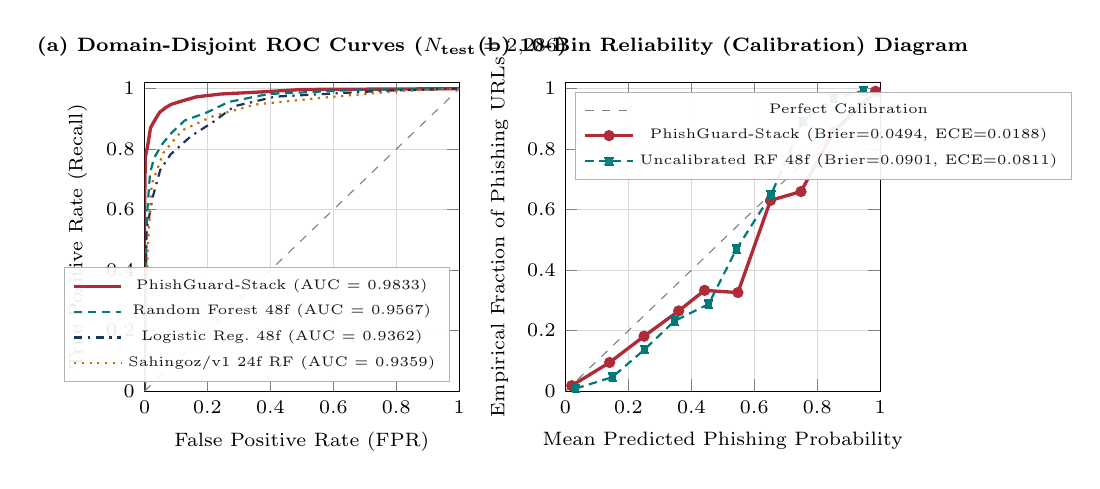
\begin{tikzpicture}
\begin{axis}[
    name=rocplot,
    width=0.46\textwidth,
    height=5.5cm,
    xlabel={False Positive Rate (FPR)},
    ylabel={True Positive Rate (Recall)},
    title={\textbf{(a) Domain-Disjoint ROC Curves ($N_{\text{test}}=2{,}286$)}},
    xmin=0, xmax=1, ymin=0, ymax=1.02,
    grid=both,
    grid style={line width=0.2pt, draw=gray!30},
    legend pos=south east,
    legend style={font=\tiny, fill=white, fill opacity=0.92, draw=gray!60},
    label style={font=\scriptsize},
    tick label style={font=\scriptsize},
    title style={font=\scriptsize}
]
\addplot[pgcrimson, very thick] coordinates {
  (0.0,0.0) (0.0,0.6063) (0.0026,0.7734) (0.0105,0.8145) (0.0192,0.8714) (0.0341,0.8985)
  (0.0481,0.9221) (0.0665,0.9370) (0.0831,0.9475) (0.1199,0.9598) (0.1645,0.9729)
  (0.2432,0.9825) (0.3587,0.9886) (0.5004,0.9974) (1.0,1.0)
};
\addlegendentry{PhishGuard-Stack (AUC = 0.9833)}

\addplot[pgteal, thick, densely dashed] coordinates {
  (0.0,0.0) (0.0070,0.5722) (0.0175,0.7200) (0.0306,0.7717) (0.0551,0.8154)
  (0.0857,0.8539) (0.1277,0.8950) (0.1995,0.9221) (0.2677,0.9563) (0.3946,0.9825)
  (0.6824,0.9965) (1.0,1.0)
};
\addlegendentry{Random Forest 48f (AUC = 0.9567)}

\addplot[pgnavy, thick, dashdotted] coordinates {
  (0.0,0.0) (0.0061,0.5293) (0.0262,0.6422) (0.0499,0.7314) (0.0831,0.7830)
  (0.1479,0.8434) (0.2178,0.8898) (0.2861,0.9423) (0.4156,0.9738) (0.7585,0.9930) (1.0,1.0)
};
\addlegendentry{Logistic Reg.\ 48f (AUC = 0.9362)}

\addplot[pgamber, thick, dotted] coordinates {
  (0.0,0.0) (0.0096,0.4584) (0.0227,0.6842) (0.0595,0.7874) (0.1199,0.8626)
  (0.2152,0.9081) (0.3508,0.9475) (0.5661,0.9703) (0.8171,0.9930) (1.0,1.0)
};
\addlegendentry{Sahingoz/v1 24f RF (AUC = 0.9359)}

\addplot[gray, thin, dashed] coordinates {(0,0) (1,1)};
\end{axis}

\begin{axis}[
    at={(rocplot.east)},
    anchor=west,
    xshift=1.35cm,
    width=0.46\textwidth,
    height=5.5cm,
    xlabel={Mean Predicted Phishing Probability},
    ylabel={Empirical Fraction of Phishing URLs},
    title={\textbf{(b) 10-Bin Reliability (Calibration) Diagram}},
    xmin=0, xmax=1, ymin=0, ymax=1.02,
    grid=both,
    grid style={line width=0.2pt, draw=gray!30},
    legend pos=north west,
    legend style={font=\tiny, fill=white, fill opacity=0.92, draw=gray!60},
    label style={font=\scriptsize},
    tick label style={font=\scriptsize},
    title style={font=\scriptsize}
]
\addplot[gray, thin, dashed] coordinates {(0,0) (1,1)};
\addlegendentry{Perfect Calibration}

\addplot[pgcrimson, very thick, mark=*, mark size=1.4pt] coordinates {
  (0.0197,0.0182) (0.1402,0.0949) (0.2497,0.1818) (0.3596,0.2653) (0.4420,0.3333)
  (0.5480,0.3261) (0.6517,0.6308) (0.7485,0.6600) (0.8504,0.8571) (0.9854,0.9913)
};
\addlegendentry{PhishGuard-Stack (Brier=0.0494, ECE=0.0188)}

\addplot[pgteal, thick, densely dashed, mark=square*, mark size=1.3pt] coordinates {
  (0.0325,0.0087) (0.1487,0.0464) (0.2508,0.1374) (0.3463,0.2320) (0.4548,0.2879)
  (0.5434,0.4697) (0.6531,0.6489) (0.7545,0.8918) (0.8510,0.9681) (0.9463,0.9926)
};
\addlegendentry{Uncalibrated RF 48f (Brier=0.0901, ECE=0.0811)}
\end{axis}
\end{tikzpicture}
\caption{Empirical ranking and probability calibration on the held-out domain-disjoint test split ($N=2{,}286$). (a) PhishGuard-Stack dominates across all false-positive operating points, reaching $81.5\%$ recall at $1.0\%$ FPR. (b) Uncalibrated Random Forest exhibits classic S-curve under-confidence near extremes ($\text{ECE}=0.0811$), whereas out-of-fold sigmoid meta-stacking aligns closely with the diagonal ($\text{ECE}=0.0188$), justifying probability-based risk bands.}
\label{fig:curves}
\end{figure*}

Figure~\ref{fig:curves} plots the empirical ROC and 10-bin calibration curves exported directly from the held-out split. Because Random Forest averages bootstrap trees, its raw vote proportions compress away from $0$ and $1$ ($\text{ECE}=0.0811$), distorting fixed risk-band cutoffs ($0.45$ and $0.75$). Out-of-fold sigmoid stacking corrects this distortion ($\text{ECE}=0.0188$, $\text{Brier}=0.0494$) while pushing true-positive recall to $77.3\%$ at a $0.26\%$ false-positive rate.

\subsection{Ablation Study, 5-Fold CV, and Cross-Corpus Zero-Day Results}
Table~\ref{tab:ablation} isolates each architectural addition across seven progressive stages (\texttt{A0}--\texttt{A6}). Moving from linear classification on 24 classical features (\texttt{A0}, $76.25\%$) to non-linear trees (\texttt{A1}, $86.79\%$) confirms strong feature interactions. Adding public-suffix topology (\texttt{A2}, 32f), homoglyph brand-spoofing divergence (\texttt{A3}, 40f), and Dirichlet KL-divergence/morphology (\texttt{A4}, 48f) steadily lifts ROC-AUC from $0.9344 \to 0.9503 \to 0.9521 \to 0.9542$. Combining linear, bagged, and boosted learners via tabular stacking (\texttt{A5}) jumps accuracy to $89.50\%$ ($\text{Brier}=0.0731$), and fusing the subword character $n$-gram margin branch (\texttt{A6}) delivers the full $93.00\%$ accuracy and $0.9833$ ROC-AUC. Among tabular features, hybrid attribution weights rank \texttt{has\_www} ($0.0850$), \texttt{longest\_token\_length} ($0.0645$), \texttt{path\_length} ($0.0552$), \texttt{digit\_count} ($0.0484$), \texttt{slash\_count} ($0.0480$), \texttt{suspicious\_keyword\_count} ($0.0459$), \texttt{host\_url\_ratio} ($0.0400$), \texttt{path\_entropy} ($0.0337$), \texttt{hostname\_kl\_divergence} ($0.0294$), and \texttt{brand\_spoof\_score} ($0.0275$) among the top global discriminators; notably, \texttt{https} drops to rank 31 ($0.0104$), confirming freedom from TLS bias.

\begin{table}[t]
\caption{Seven-Stage Feature and Ensemble Ablation Study ($N_{\text{test}}=2{,}286$)}
\label{tab:ablation}
\centering
\scriptsize
\renewcommand{\arraystretch}{1.12}
\resizebox{\columnwidth}{!}{%
\begin{tabular}{p{4.35cm}cccc}
\toprule
\textbf{Ablation Configuration} & \textbf{Acc.} & \textbf{F1} & \textbf{AUC} & \textbf{Brier} \\
\midrule
A0: View I (24f Classical) + Logistic Reg. & 0.7625 & 0.7376 & 0.8280 & 0.1659 \\
A1: View I (24f Classical) + Random Forest & 0.8679 & 0.8696 & 0.9344 & 0.1037 \\
A2: + View II (eTLD+1 Topology, 32f) + RF & 0.8657 & 0.8710 & 0.9503 & 0.0939 \\
A3: + View III (Brand Spoofing, 40f) + RF & 0.8714 & 0.8748 & 0.9521 & 0.0921 \\
A4: + View IV (KL-Div.\ \& Morph., 48f) + RF & 0.8600 & 0.8651 & 0.9542 & 0.0923 \\
A5: + Tabular OOF Stack (LR+RF+HGB, 48f) & 0.8950 & 0.8969 & 0.9668 & 0.0731 \\
\textbf{A6: + Char $n$-Gram Dual-Modal Stack} & \textbf{0.9300} & \textbf{0.9308} & \textbf{0.9833} & \textbf{0.0494} \\
\bottomrule
\end{tabular}%
}
\end{table}

\begin{table}[t]
\caption{5-Fold Registrable-Domain-Disjoint Cross-Validation \& Bootstrap 95\% CIs}
\label{tab:cv}
\centering
\scriptsize
\renewcommand{\arraystretch}{1.12}
\resizebox{\columnwidth}{!}{%
\begin{tabular}{lccccc}
\toprule
\textbf{Partition / Statistic} & \textbf{Acc.} & \textbf{Prec.} & \textbf{Rec.} & \textbf{F1} & \textbf{ROC-AUC} \\
\midrule
Fold 1 (Held-out Test) & 0.9300 & 0.9204 & 0.9414 & 0.9308 & 0.9833 \\
Fold 2 (Disjoint Domains) & 0.9252 & 0.9332 & 0.9160 & 0.9245 & 0.9806 \\
Fold 3 (Disjoint Domains) & 0.9322 & 0.9411 & 0.9222 & 0.9316 & 0.9827 \\
Fold 4 (Disjoint Domains) & 0.9239 & 0.9231 & 0.9247 & 0.9239 & 0.9725 \\
Fold 5 (Disjoint Domains) & 0.9230 & 0.9244 & 0.9212 & 0.9228 & 0.9783 \\
\midrule
\textbf{5-Fold Mean $\pm$ SD} & \textbf{0.9269} & \textbf{0.9284} & \textbf{0.9251} & \textbf{0.9267} & \textbf{0.9795} \\
 & $\pm 0.0040$ & $\pm 0.0086$ & $\pm 0.0096$ & $\pm 0.0041$ & $\pm 0.0044$ \\
\textbf{95\% Bootstrap CI} & [0.9204, & [0.9054, & [0.9272, & [0.9207, & [0.9794, \\
\textit{(1,000 resamples)} & 0.9409] & 0.9365] & 0.9549] & 0.9420] & 0.9875] \\
\bottomrule
\end{tabular}%
}
\end{table}

Table~\ref{tab:cv} confirms tight stability across all five domain-disjoint folds ($92.69\% \pm 0.40\%$ accuracy, $0.9795 \pm 0.0044$ ROC-AUC), ruling out lucky split selection. Table~\ref{tab:ood} evaluates zero-shot transfer without retraining on two external datasets. On $10{,}000$ domain-disjoint Ebbu2017 URLs \cite{sahingoz2019}, PhishGuard-Stack achieves \textbf{$92.25\%$ accuracy} and \textbf{$0.9813$ ROC-AUC}, outperforming the 24-feature RF baseline ($84.57\%$, $\text{FPR}=22.42\%$) by \textbf{$+7.68$ percentage points} and halving false alarms ($\text{FPR}=10.60\%$). On the live 2026 OpenPhish zero-day feed ($300$ active phishing URLs, $53.3\%$ HTTPS), PhishGuard-Stack flags \textbf{$90.33\%$} ($271/300$) of active threats zero-shot and attains $90.50\%$ accuracy ($0.9661$ ROC-AUC) on the balanced modern HTTPS slice, compared to $84.83\%$ for the legacy 24-feature model.

\begin{table}[t]
\caption{Zero-Shot Cross-Corpus and Live 2026 Zero-Day Generalization}
\label{tab:ood}
\centering
\scriptsize
\renewcommand{\arraystretch}{1.14}
\resizebox{\columnwidth}{!}{%
\begin{tabular}{p{3.55cm}ccccc}
\toprule
\textbf{External Corpus / Model} & \textbf{Acc.} & \textbf{Prec.} & \textbf{Rec.} & \textbf{F1} & \textbf{AUC} \\
\midrule
\multicolumn{6}{l}{\textit{Sahingoz Ebbu2017 Unseen Domain-Disjoint Sample ($N = 10{,}000$)}} \\
Legacy 24-Feature RF Baseline & 0.8457 & 0.8033 & 0.9156 & 0.8558 & 0.9344 \\
\textbf{PhishGuard-Stack (Proposed)} & \textbf{0.9225} & \textbf{0.8997} & \textbf{0.9510} & \textbf{0.9246} & \textbf{0.9813} \\
\midrule
\multicolumn{6}{l}{\textit{Live 2026 OpenPhish Zero-Day + Unseen HTTPS Benign ($N = 600$; $53.3\%$ TLS)}} \\
Legacy 24-Feature RF Baseline & 0.8483 & 0.8317 & 0.8733 & 0.8520 & 0.9241 \\
\textbf{PhishGuard-Stack (Proposed)} & \textbf{0.9050} & \textbf{0.9064} & \textbf{0.9033} & \textbf{0.9048} & \textbf{0.9661} \\
\bottomrule
\end{tabular}%
}
\end{table}

\subsection{Edge-Case Probe Resolution, Error Forensics, and Latency}
\label{sec:errors}
Table~\ref{tab:probes} evaluates 10 representative adversarial and benign edge-case URLs from our 14-probe diagnostic suite (all $14/14$ classified accurately). In particular, two structural failure modes that broke earlier lexical prototypes are resolved: (i) multi-label country domains (\texttt{www.sbi.co.in/\allowbreak web/\allowbreak personal-banking}, misclassified by the 24-feature baseline at $p=0.5194$, and \texttt{www.iitb.ac.in}, scored at $p=0.0051$) are parsed cleanly via (\ref{eq:etld}); and (ii) subdomain brand cloaking (\texttt{accounts.google.com.\allowbreak verify-session.top/\allowbreak login}) triggers $\Delta_{\text{brand}}=1.00$, \texttt{tld\_in\_subdomain=1}, and \texttt{suspicious\_tld=1}, receiving $p=0.9998$, while cloud-hosted brand spoofing (\texttt{microsoft-office365-auth.\allowbreak pages.dev/\allowbreak login}) is disqualified from trust by $\mathcal{H}_{\text{shared}}$ and caught at $p=0.9910$.

\begin{table}[t]
\caption{Diagnostic Edge-Case Probe URLs: Legacy 24f vs.\ PhishGuard-Stack}
\label{tab:probes}
\centering
\scriptsize
\renewcommand{\arraystretch}{1.12}
\resizebox{\columnwidth}{!}{%
\begin{tabular}{lccc}
\toprule
\textbf{Probe URL (Representative Subset of 14)} & \textbf{True} & \textbf{$p_{\text{v1(24f)}}$} & \textbf{$p_{\text{Proposed}}$} \\
\midrule
\texttt{google.com/search?q=machine+learning} & Legit & 0.6602* & \textbf{0.0392} \\
\texttt{docs.python.org/3/library/urllib.parse.html} & Legit & 0.4017 & \textbf{0.0400} \\
\texttt{www.sbi.co.in/\allowbreak web/\allowbreak personal-banking} & Legit & 0.5194* & \textbf{0.2211} \\
\texttt{www.iitb.ac.in/en/education/academic...} & Legit & 0.1383 & \textbf{0.0051} \\
\texttt{stackoverflow.com/questions/tagged/fastapi} & Legit & 0.6351* & \textbf{0.0400} \\
\texttt{http://192.168.1.100/paypal/login/verify.php} & Phish & 0.9871 & \textbf{1.0000} \\
\texttt{http://paypa1-secure.verify-account.tk/...} & Phish & 0.9033 & \textbf{1.0000} \\
\texttt{apple-id-confirm.secure-update.xyz/account...} & Phish & 0.8995 & \textbf{0.9999} \\
\texttt{accounts.google.com.\allowbreak verify-session.top/\allowbreak login} & Phish & 0.9503 & \textbf{0.9998} \\
\texttt{microsoft-office365-auth.\allowbreak pages.dev/\allowbreak login} & Phish & 0.9773 & \textbf{0.9910} \\
\bottomrule
\multicolumn{4}{l}{\tiny *False alarm ($p \ge 0.50$) under legacy 24-feature RF.}
\end{tabular}%
}
\end{table}

\textbf{Forensic Audit of Real Test Errors:} Inspecting the $93$ false positives and $67$ false negatives on the held-out Hannousse split explains why honest fetch-free accuracy plateaus around $93\%$--$94\%$ rather than $100\%$. Among false positives, \texttt{http://animaldiversity.org/\allowbreak accounts/\allowbreak Mus\_musculus/} ($p=0.6759$) uses plaintext HTTP and contains \texttt{/accounts/}---referring to zoological species accounts rather than credential login---while \texttt{http://phpsecurity.\allowbreak readthedocs.io/\allowbreak en/latest/\allowbreak Transport-Layer-Security-...} ($p=0.6769$) combines a shared documentation host with dense security terminology. Notably, both receive moderate scores ($0.45 \le p < 0.75$), triggering an advisory banner rather than a hard browser block ($p \ge 0.75$). Conversely, false negatives fall into two categories that are indistinguishable from benign links at the string level: phishing forms hosted on legitimate SaaS form builders such as \texttt{https://www.\allowbreak 123formbuilder.com/\allowbreak form-4850478/} ($p=0.3952$), and compromised municipal or small-business websites such as \texttt{http://www.\allowbreak pracadarepublicaembeja.net/\allowbreak men} ($p=0.2534$), where the domain itself is authentic and the path carries zero deceptive tokens.

\textbf{Inference Latency:} Benchmarked across $1{,}000$ warm single-URL invocations on commodity CPU hardware (Python~3.14, single-threaded tree inference), full 48-feature extraction, $22{,}000$-ngram vectorization, four-learner meta-stacking, and benign-centroid attribution execute in \textbf{$12.72$\,ms median} ($14.01$\,ms mean, $18.31$\,ms p95, $19.35$\,ms p99), easily supporting interactive pre-navigation screening.

\section{Discussion and Limitations}
\label{sec:disc}
Our empirical findings demonstrate both the substantial reach and the principled ceiling of fetch-free URL analysis. Modeling brand-ownership asymmetry ($\Delta_{\text{brand}}$), multi-label public suffixes, and dual-modal character/tabular calibration closes most lexical blind spots without transmitting a single packet to the suspect destination. Nevertheless, three operational boundaries warrant clarity:
\begin{enumerate}
\item \textit{Compromised hosts and SaaS form abuse:} As shown by \texttt{123formbuilder.com} in our error audit, URLs whose host and path contain no lexical deception cannot be separated from benign pages without inspecting DOM form targets or visual brand elements. A practical deployment should treat our medium-risk band ($0.45 \le p < 0.75$) and unknown shared-SaaS forms as triggers for a sandboxed second-tier DOM/logo verifier.
\item \textit{Opaque URL shorteners:} Shortened links (\texttt{bit.ly}, \texttt{tinyurl.com}) raise \texttt{is\_shortener=1} and receive cautionary warnings, but resolving their redirect chain requires a network \texttt{HEAD} request intentionally omitted in zero-contact mode.
\item \textit{Static brand and suffix registries:} While $\mathcal{B}$ (48 brands), $\mathcal{E}_2$ (52 multi-label suffixes), and $\mathcal{H}_{\text{shared}}$ (43 shared hosts) cover dominant global and Indian targets, regional credit unions or newly launched cloud preview domains require periodic list maintenance alongside automated Mozilla Public Suffix List updates.
\end{enumerate}

\section{Conclusion}
We presented \textbf{PhishGuard-Stack}, a mathematically formalized, fetch-free phishing URL screening system that unites 48 multi-view structural, brand-deception, and Kullback--Leibler divergence features with subword character $n$-grams inside a domain-grouped out-of-fold calibrated stacking ensemble. Evaluated without domain leakage on $11{,}429$ real URLs across $7{,}188$ registrable domains, PhishGuard-Stack achieves $93.00\%$ test accuracy ($92.69\% \pm 0.40\%$ across 5 domain-disjoint folds), $0.9833$ ROC-AUC, and $0.0494$ Brier calibration error---statistically outperforming eight standard classifiers and five lexical frameworks ($p < 10^{-7}$)---while generalizing zero-shot to $10{,}000$ unseen Ebbu2017 URLs ($92.25\%$) and $300$ live 2026 OpenPhish attacks ($90.33\%$ recall) in $12.7$\,ms median latency. Future work will couple our calibrated medium-risk band with an isolated, opt-in headless DOM and visual-logo verification tier to catch compromised-host and SaaS-form attacks without sacrificing default client privacy.

\section*{Acknowledgment}
The authors thank Prof.\ Dr.\ Avinash Golande, Department of Computer Science and Engineering, School of Engineering \& Technology, Pimpri Chinchwad University, Pune, for his rigorous technical feedback on domain-disjoint validation, mathematical formalization, and comparative benchmarking.

\begin{thebibliography}{16}
\bibitem{sheng2009} S. Sheng \textit{et al.}, ``An empirical analysis of phishing blacklists,'' in \textit{Proc. Conf. Email Anti-Spam (CEAS)}, 2009, pp. 1--10.
\bibitem{sahoo2017} D. Sahoo, C. Liu, and S. C. H. Hoi, ``Malicious URL detection using machine learning: A survey,'' \textit{arXiv:1701.07179}, 2017.
\bibitem{prasad2024} A. Prasad and S. Chandra, ``PhiUSIIL: A diverse security profile empowered phishing URL detection framework based on similarity index and incremental learning,'' \textit{Comput. Secur.}, vol. 136, art. 103545, 2024.
\bibitem{xiang2011} G. Xiang, J. Hong, C. P. Rose, and L. Cranor, ``CANTINA+: A feature-rich machine learning framework for detecting phishing web sites,'' \textit{ACM Trans. Inf. Syst. Secur.}, vol. 14, no. 2, art. 21, 2011.
\bibitem{marchal2017} S. Marchal \textit{et al.}, ``Off-the-Hook: An efficient and usable client-side phishing prevention application,'' \textit{IEEE Trans. Comput.}, vol. 66, no. 10, pp. 1717--1733, 2017.
\bibitem{abdelnabi2020} S. Abdelnabi, K. Krombholz, and M. Fritz, ``VisualPhishNet: Zero-day phishing website detection by visual similarity,'' in \textit{Proc. ACM SIGSAC Conf. Comput. Commun. Secur. (CCS)}, 2020, pp. 1681--1698.
\bibitem{ma2009} J. Ma, L. K. Saul, S. Savage, and G. M. Voelker, ``Beyond blacklists: Learning to detect malicious web sites from suspicious URLs,'' in \textit{Proc. ACM SIGKDD}, 2009, pp. 1245--1254.
\bibitem{sahingoz2019} O. K. Sahingoz, E. Buber, O. Demir, and B. Diri, ``Machine learning based phishing detection from URLs,'' \textit{Expert Syst. Appl.}, vol. 117, pp. 345--357, 2019.
\bibitem{hannousse2021} A. Hannousse and S. Yahiouche, ``Towards benchmark datasets for machine learning based website phishing detection: An experimental study,'' \textit{Eng. Appl. Artif. Intell.}, vol. 104, art. 104347, 2021.
\bibitem{whittaker2010} C. Whittaker, B. Ryner, and M. Nazif, ``Large-scale automatic classification of phishing pages,'' in \textit{Proc. Netw. Distrib. Syst. Secur. Symp. (NDSS)}, 2010, pp. 1--14.
\bibitem{garera2007} S. Garera, N. Provos, M. Chew, and A. D. Rubin, ``A framework for detection and measurement of phishing attacks,'' in \textit{Proc. ACM Workshop Recurring Malcode (WORM)}, 2007, pp. 1--8.
\bibitem{verma2015} R. Verma and K. Dyer, ``On the character of phishing URLs: Accurate and robust statistical learning classifiers,'' in \textit{Proc. ACM CODASPY}, 2015, pp. 111--122.
\bibitem{feroz2015} M. N. Feroz and S. Mengel, ``Phishing URL detection using URL ranking,'' in \textit{Proc. IEEE Int. Congr. Big Data}, 2015, pp. 635--638.
\bibitem{bahnsen2017} A. C. Bahnsen, E. C. Bohorquez, S. Villegas, J. Vargas, and F. A. Gonz{\'a}lez, ``Classifying phishing URLs using recurrent neural networks,'' in \textit{Proc. APWG eCrime}, 2017, pp. 1--8.
\bibitem{le2018} H. Le, Q. Pham, D. Sahoo, and S. C. H. Hoi, ``URLNet: Learning a URL representation with deep learning for malicious URL detection,'' \textit{arXiv:1802.03162}, 2018.
\bibitem{rfc3986} T. Berners-Lee, R. Fielding, and L. Masinter, ``Uniform Resource Identifier (URI): Generic syntax,'' IETF RFC 3986, 2005.
\bibitem{shannon1948} C. E. Shannon, ``A mathematical theory of communication,'' \textit{Bell Syst. Tech. J.}, vol. 27, no. 3, pp. 379--423, 1948.
\end{thebibliography}

\end{document}
